\documentclass{beamer}
\usepackage[utf8]{inputenc}
\usetheme{Madrid}
\usecolortheme{default}
\usepackage{amsmath,amssymb,amsfonts,amsthm}
\usepackage{txfonts}
\usepackage{tkz-euclide}
\usepackage{listings}
\usepackage{adjustbox}
\usepackage{array}
\usepackage{tabularx}
\usepackage{gvv}
\usepackage{lmodern}
\usepackage{circuitikz}
\usepackage{tikz}
\usepackage{graphicx}

\setbeamertemplate{page number in head/foot}[totalframenumber]

\usepackage{tcolorbox}
\tcbuselibrary{minted,breakable,xparse,skins}



\definecolor{bg}{gray}{0.95}
\DeclareTCBListing{mintedbox}{O{}m!O{}}{%
  breakable=true,
  listing engine=minted,
  listing only,
  minted language=#2,
  minted style=default,
  minted options={%
    linenos,
    gobble=0,
    breaklines=true,
    breakafter=,,
    fontsize=\small,
    numbersep=8pt,
    #1},
  boxsep=0pt,
  left skip=0pt,
  right skip=0pt,
  left=25pt,
  right=0pt,
  top=3pt,
  bottom=3pt,
  arc=5pt,
  leftrule=0pt,
  rightrule=0pt,
  bottomrule=2pt,
  toprule=2pt,
  colback=bg,
  colframe=orange!70,
  enhanced,
  overlay={%
    \begin{tcbclipinterior}
    \fill[orange!20!white] (frame.south west) rectangle ([xshift=20pt]frame.north west);
    \end{tcbclipinterior}},
  #3,
}
\lstset{
    language=C,
    basicstyle=\ttfamily\small,
    keywordstyle=\color{blue},
    stringstyle=\color{orange},
    commentstyle=\color{green!60!black},
    numbers=left,
    numberstyle=\tiny\color{gray},
    breaklines=true,
    showstringspaces=false,
}
%------------------------------------------------------------
%This block of code defines the information to appear in the
%Title page
\title %optional
{4.13.85-Beamer}

%\subtitle{A short story}

\author % (optional)
{Varun-ai25btech11016}



\begin{document}


\frame{\titlepage}
\begin{frame}{Question}
If the lines $\dfrac{x-1}{2} = \dfrac{y+1}{3} = \dfrac{z-1}{4}$ 
and $\dfrac{x-3}{1} = \dfrac{y-k}{2} = \dfrac{z}{1}$ intersect, 
then the value of $k$ is

\end{frame}
\begin{frame}{Theoretical solution}
The lines $A+ K_1m_1,B+K_2m_2$ will intersect if 
\begin{align}
\operatorname{rank}(\vec{M} \hspace{5mm}  \vec{B-A})&=2\\
\vec{M}=\myvec{m_1&&m_2}\\
\end{align}
Here,
\begin{align}
\vec{m_1}=\myvec{2\\3\\4} \vec{m_2}=\myvec{1\\2\\1}
\end{align}
\end{frame}
\begin{frame}{Theoretical solution}

\begin{align}
\vec{M}&=\myvec{2&&1\\3&&2\\4&&1}\\
\vec{A}&=\myvec{1\\-1\\1} ,\vec{B}=\myvec{3\\k\\0}\\
\vec{B-A}&=\myvec{3-1\\k-(-1)\\-1}=\myvec{2\\k+1\\-1}\\
\operatorname{rank}\Bigg(\myvec{2&&1&&2\\3&&2&&k+1\\4&&1&&-1}\Bigg)&=2
\end{align}

\end{frame}
\begin{frame}{Theoretical solution}
\begin{align}
\begin{pmatrix}
2 & 1 & 2\\
3 & 2 & k+1\\
4 & 1 & -1
\end{pmatrix}
\;\xrightarrow[\;R_3 \to 2R_3 - 4R_1\;]{\;R_2 \to 2R_2 - 3R_1\;}\;
\begin{pmatrix}
2 & 1 & 2\\
0 & 1 & 2k-4\\
0 & -2 & -10
\end{pmatrix}\\
\;\\\xrightarrow[\;]{\;R_3 \to R_3 + 2R_2\;}\;
\begin{pmatrix}
2 &1 & 2\\
0 & 1 & 2k-4\\
0 & 0 & 4k-18
\end{pmatrix}\end{align}
For the$ \operatorname{rank}(\vec{M} \hspace{5mm}  \vec{B-A})$ to be 2\\
the last row must be all zero implies\\
\begin{align}
4k-18&=0\\
k&=\tfrac{9}{2}
\end{align}
\end{frame}
\begin{frame}[fragile]
    \frametitle{C code}
    \begin{lstlisting}
    #include <stdlib.h>

// Fill arrays with coordinates of Line 1: (1+2t, -1+3t, 1+4t)
// and Line 2: (3+t, k+2t, t)
// Inputs: t_min, t_max, n_points, k
// Outputs: arrays (x1,y1,z1,x2,y2,z2)
void generate_lines(double t_min, double t_max, int n_points, double k,
                    double *x1, double *y1, double *z1,
                    double *x2, double *y2, double *z2) {
    double step = (t_max - t_min) / (n_points - 1);

    for (int i = 0; i < n_points; i++) {
        double t = t_min + i * step;
        \end{lstlisting}
\end{frame}
\begin{frame}[fragile]
    \frametitle{C code}
    \begin{lstlisting}
        // Line 1
        x1[i] = 1 + 2*t;
        y1[i] = -1 + 3*t;
        z1[i] = 1 + 4*t;

        // Line 2
        x2[i] = 3 + t;
        y2[i] = k + 2*t;
        z2[i] = t;
    }
}
 \end{lstlisting}
\end{frame}
\begin{frame}[fragile]
    \frametitle{Py with C code}
    \begin{lstlisting}
import ctypes
import numpy as np
import matplotlib.pyplot as plt

# Load the shared library
lib = ctypes.CDLL("./liblines.so")

# Define function signature
lib.generate_lines.argtypes = [
    ctypes.c_double, ctypes.c_double, ctypes.c_int, ctypes.c_double,
    np.ctypeslib.ndpointer(dtype=np.float64, ndim=1, flags="C_CONTIGUOUS"),
    np.ctypeslib.ndpointer(dtype=np.float64, ndim=1, flags="C_CONTIGUOUS"),
    np.ctypeslib.ndpointer(dtype=np.float64, ndim=1, flags="C_CONTIGUOUS"),
     \end{lstlisting}
\end{frame}
\begin{frame}[fragile]
    \frametitle{Py with C code}
    \begin{lstlisting}
np.ctypeslib.ndpointer(dtype=np.float64, ndim=1, flags="C_CONTIGUOUS"),
    np.ctypeslib.ndpointer(dtype=np.float64, ndim=1, flags="C_CONTIGUOUS"),
    np.ctypeslib.ndpointer(dtype=np.float64, ndim=1, flags="C_CONTIGUOUS"),
]
lib.generate_lines.restype = None

# Parameters
n_points = 200
t_min, t_max = -10, 10
k = 2.0  # change this as needed
 \end{lstlisting}
\end{frame}
\begin{frame}[fragile]
    \frametitle{Py with C code}
    \begin{lstlisting}

# Allocate numpy arrays
x1 = np.zeros(n_points, dtype=np.float64)
y1 = np.zeros(n_points, dtype=np.float64)
z1 = np.zeros(n_points, dtype=np.float64)
x2 = np.zeros(n_points, dtype=np.float64)
y2 = np.zeros(n_points, dtype=np.float64)
z2 = np.zeros(n_points, dtype=np.float64)
 \end{lstlisting}
\end{frame}
\begin{frame}[fragile]
    \frametitle{Py with C code}
    \begin{lstlisting}

# Call C function
lib.generate_lines(t_min, t_max, n_points, k, x1, y1, z1, x2, y2, z2)

# Plot 3D
fig = plt.figure(figsize=(10, 7))
ax = fig.add_subplot(111, projection="3d")

ax.plot(x1, y1, z1, label="Line 1", color="blue")
ax.plot(x2, y2, z2, label=f"Line 2 (k={k})", color="orange")
 \end{lstlisting}
\end{frame}
\begin{frame}[fragile]
    \frametitle{Py with C code}
    \begin{lstlisting}

ax.scatter(x1[0], y1[0], z1[0], color="red", s=50, label="Start Line 1")
ax.scatter(x2[0], y2[0], z2[0], color="green", s=50, label="Start Line 2")

ax.set_xlabel("X-axis")
ax.set_ylabel("Y-axis")
ax.set_zlabel("Z-axis")
ax.set_title("3D Plot of Two Lines (from C library)")
ax.legend()
plt.show()
 \end{lstlisting}
\end{frame}
\begin{frame}[fragile]
    \frametitle{Py code}
    \begin{lstlisting}
import numpy as np
import matplotlib.pyplot as plt
from mpl_toolkits.mplot3d import Axes3D

# Parameter range
t = np.linspace(-10, 10, 200)

# First line: (x, y, z) = (1+2λ, -1+3λ, 1+4λ)
x1 = 1 + 2*t
y1 = -1 + 3*t
z1 = 1 + 4*t

# Second line: (x, y, z) = (3+μ, k+2μ, μ)
# Example: set k = 2 (you can change it to the value you solve for)
k = 2
x2 = 3 + t
y2 = k + 2*t
z2 = t
 \end{lstlisting}
\end{frame}
\begin{frame}[fragile]
    \frametitle{Py code}
    \begin{lstlisting}

# Create 3D plot
fig = plt.figure(figsize=(10, 7))
ax = fig.add_subplot(111, projection='3d')

# Plot lines
ax.plot(x1, y1, z1, label="Line 1", color="blue")
ax.plot(x2, y2, z2, label=f"Line 2 (k={k})", color="orange")

# Mark reference points
ax.scatter(1, -1, 1, color='red', s=50, label="Point on Line 1")
ax.scatter(3, k, 0, color='green', s=50, label="Point on Line 2")
 \end{lstlisting}
\end{frame}
\begin{frame}[fragile]
    \frametitle{Py code}
    \begin{lstlisting}

# Labels & title
ax.set_xlabel("X-axis")
ax.set_ylabel("Y-axis")
ax.set_zlabel("Z-axis")
ax.set_title("3D Plot of Two Lines")
ax.legend()
plt.show()
\end{lstlisting}
\end{frame}
\begin{frame}{plot}
\begin{figure}[h]
    \centering
    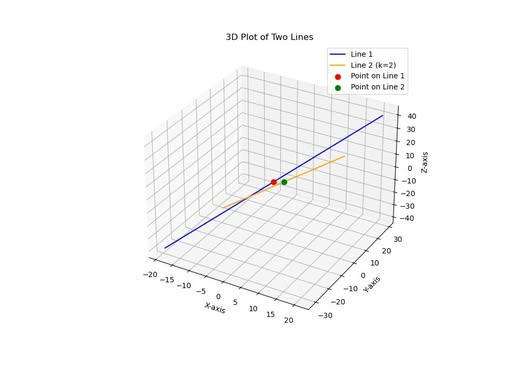
\includegraphics[scale=0.5]{figs/4.13.85.png}
    \caption{}
    \label{fig:1}
\end{figure}
\end{frame}
\end{document}